\section{Redis}

Redis (Remote Dictionary Service) merupakan basis data \textit{open-source} berbasiskan \textit{key-value store}. Redis mendukung berbagai tipe data, mulai dari string, bitmap, bitfield, hash, list, set, hingga stream. Selain itu, Redis merupakan basis data yang menyimpan data pada memori (\textit{in-memory}) dan berjalan secara \textit{single thread} sehingga Redis berjalan dengan cepat dan tidak perlu memikirkan konkurensi. Selain itu, Redis memiliki banyak dukungan fitur seperti dukungan \textit{persistence} dengan \textit{snapshot} atau \textit{append-only file} (AOF), dukungan \textit{high-availability}, replikasi, \textit{sharding}, \textit{pubsub}, \textit{stream}, dan lain-lain \parencite{redisExplained}.

\begin{figure}[htbp]
    \centering
    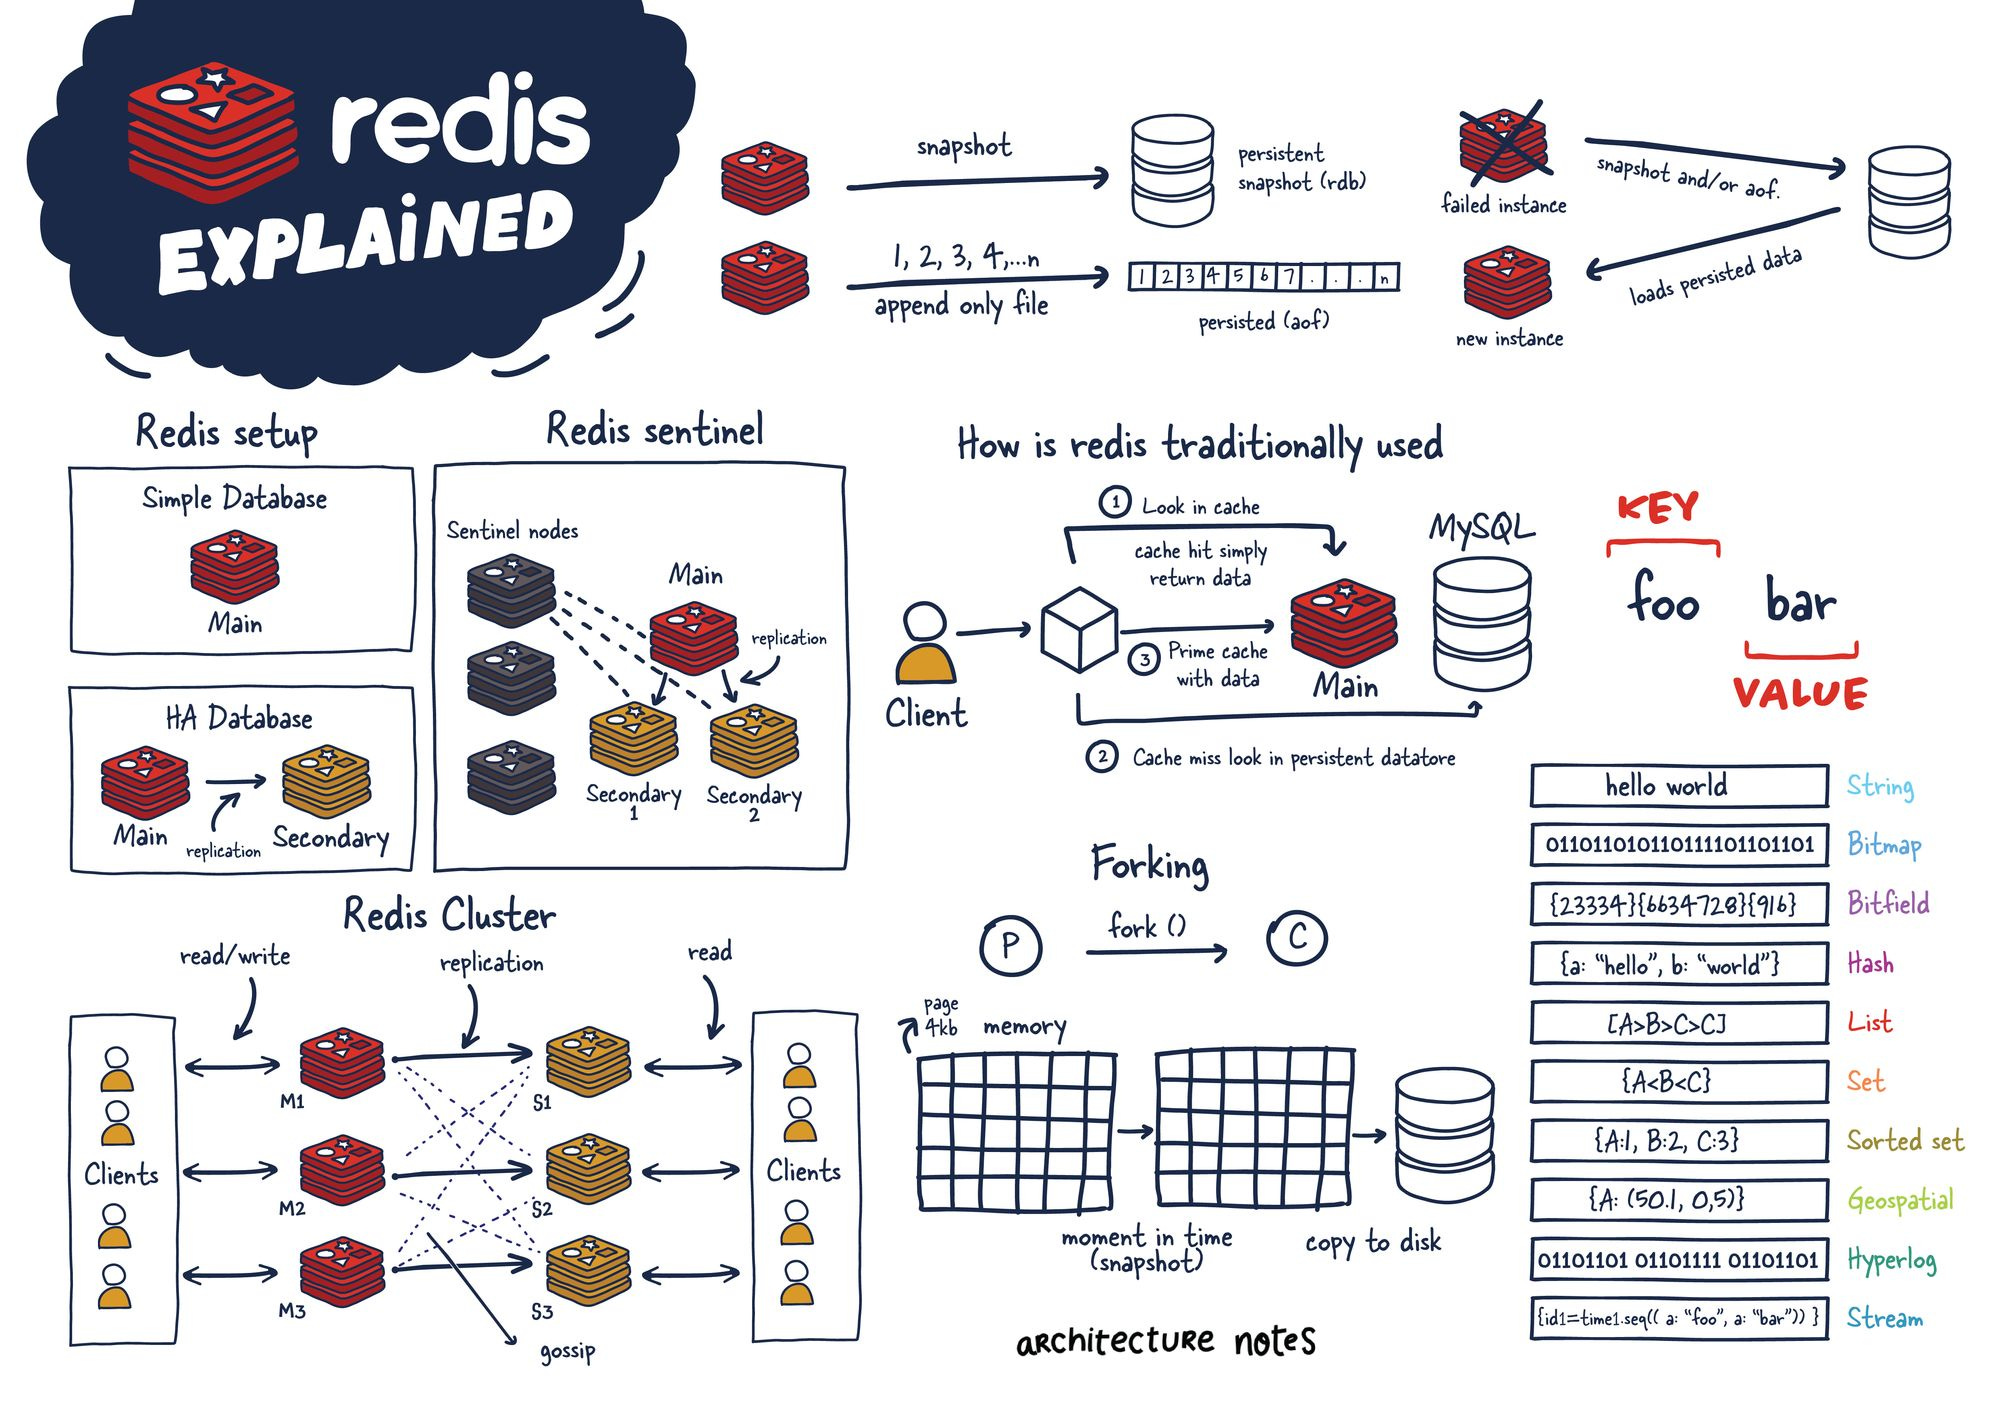
\includegraphics[width=1\textwidth]{resources/chapter-2/redis.jpg}
    \caption{\textit{Redis Explained \parencite{redisExplained}}}
    \label{fig:redis-explained}
\end{figure}

Konfigurasi Redis Cluster memungkinkan penskalaan secara horizontal dengan menyebarkan data pada mesin (\textit{sharding}). Redis menggunakan fungsi hash deterministik untuk mendistribusikan data. Selain itu, Redis menggunakan \textit{gossip protocol} untuk menilai keadaan kluster. Ketika \textit{master} tidak responsif, node \textit{secondary} dapat dipromosikan menjadi node \textit{primary} \parencite{redisExplained}.